\documentclass[12pt]{article}
\usepackage[utf8]{inputenc}
\usepackage{graphicx}

\newcommand{\co}[1]{\texttt{#1}}

\title{Poshex}
\author{Paul Răzvan Nechifor, Master ISS, an I}

\begin{document}
\maketitle

\tableofcontents
\pagebreak

\section*{Introduction}
\addcontentsline{toc}{section}{Introduction}

Poshex is an extension for Google Chrome which scans visited pages for semantic
markup formats (Microdata, RDFa and microformats) and signals the presence by
showing an icon in the address bar.

Like modern extensions, it is intended to be unobtrusive and lightweight. It
only scans the page to detect the presence of each format and it only parses and
converts the data when selected.

\begin{figure}[b!]
    \centering
    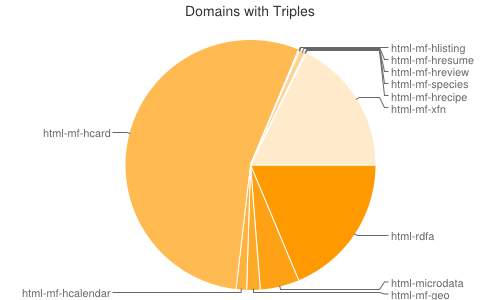
\includegraphics[width=10cm]{uf-chart}
    \caption{Microformats made up 70~\% of structured data domains in Q1/Q2
    2012\cite{ufStat}.}
\end{figure}


When selected it opens a new tab which shows:
\begin{itemize}
    \item the autoformatted page source code with attributes specific to
    Microdata and RDFa being  highlighted;
    \item for each of the detected formats, the scanner specific data format;
    \item RDF/XML conversion (for all);
    \item Turtle conversion (for Microdata and RDFa);
    \item CSV conversion for Microdata;
    \item a graph for microformats;
    \item a table view for Microdata.
\end{itemize}

All the text formats shown are syntax highlighted and can be saved locally.

The purpose of this extension is to give developers the posibility to visualize
and inspect web pages with structured data.

\section{State of the art}

\subsection{Microformats}

Microformats were invented in 2004\cite{ufHist} as a way to markup data
semantically in order to extend the sematic capabilities of regular HTML.
Microformats use reduce/reuse/recycle design principles and as such, they use
existing HTML attributes to add sematic meaning\cite{ufWiki}.

Microformats are the oldest of the three formats presented here and the most
used acording to a Web Data Commons crawl statistics\cite{ufStat}.

\begin{figure}[b!]
    \centering
    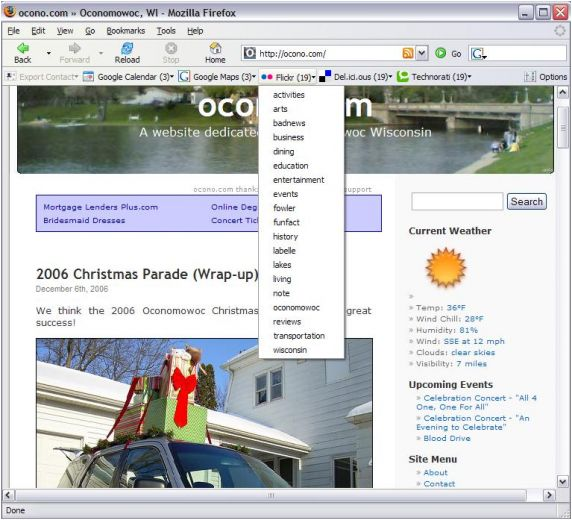
\includegraphics[width=8cm]{uf-operator}
    \caption{Operator example from its download page.}
\end{figure}


Being the oldest, microformats also have the most problems:
\begin{itemize}
    \item reusing the class attribute with a different meaning can cause
    problems because it's hard to tell which classes are intended for CSS
    presentation and which are for data markup;
    \item microformats can't be extended by just everyone, class names must be
    standardised in order for them to be detected;
    \item they are hard to parse since you have to know all the class names for
    every microformat in order to detect them.
\end{itemize}

\noindent
Browser extensions for microformats:
\begin{description}
    \item[Operator] is a Firefox plugin which reveals and provides easy access
    to microformats that are all over numerous websites.\cite{ufExt} It's
    architecture for parsing microformats has been incorporated in Firefox since
    version 3. Operator allows the user the combine information from different
    sources in a useful way (Flickr+Google Maps, Yahoo! Local + Outlook).
    \item[Google Maps for Microformats] Firefox plugin adds a context menu item
    for viewing places on Google Maps by using the adr and geo microformats.
    \item[Microformats for Google Chrome] is an extension which adds a popup
    page which shows styled detected microformats.
\end{description}

\begin{figure}[b!]
    \centering
    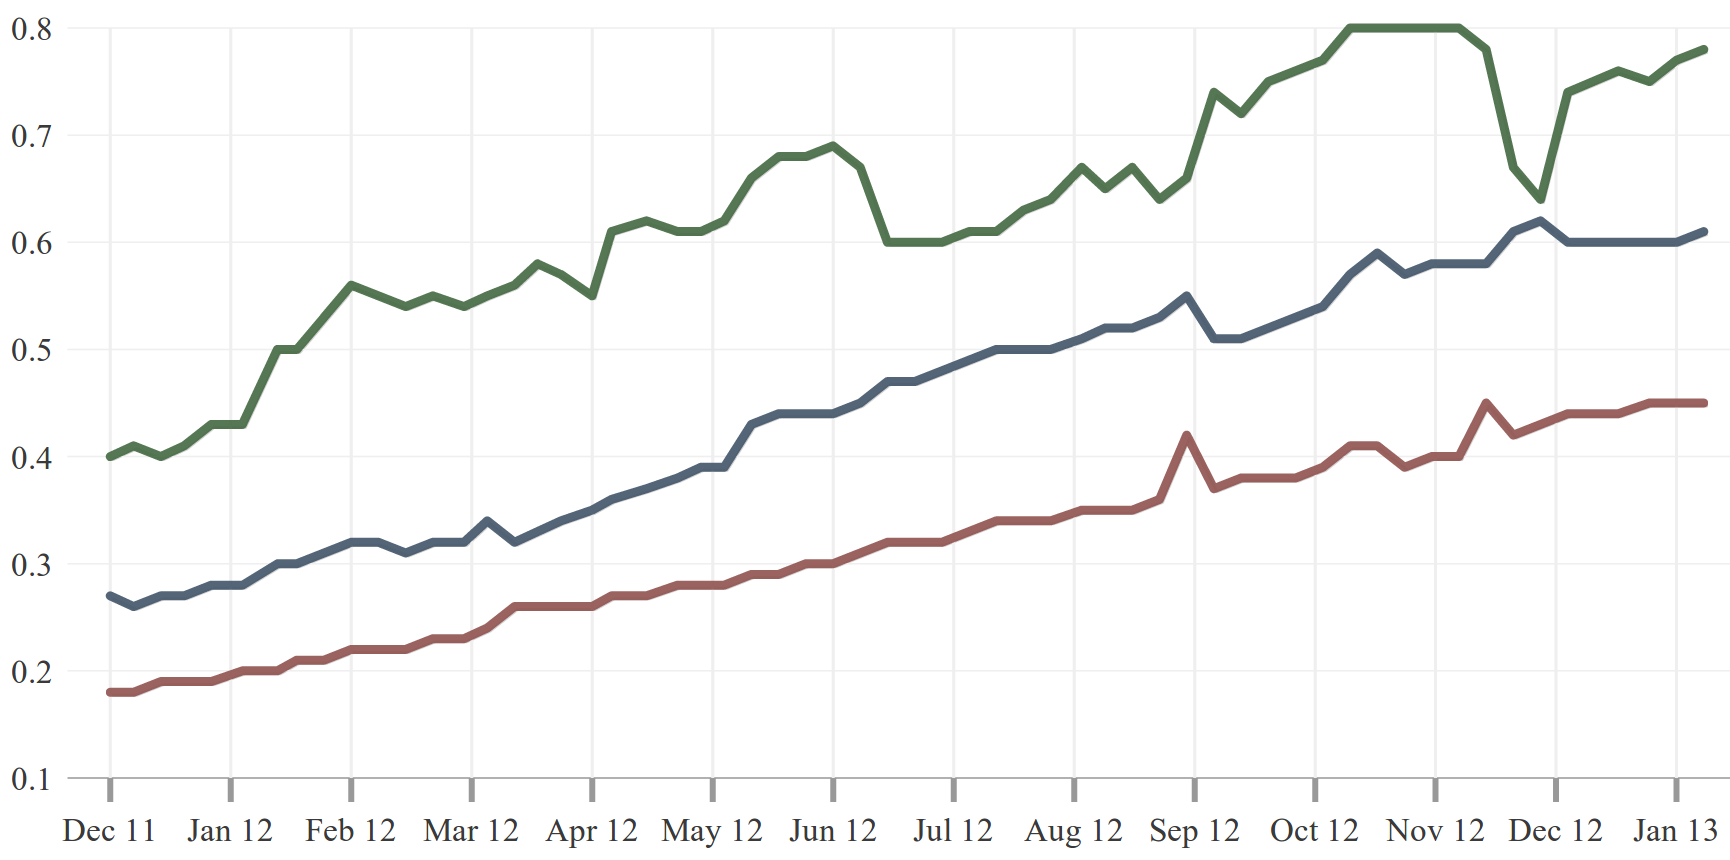
\includegraphics[width=13cm]{rdfa-chart}
    \caption{Usage statistics for RDFa.\cite{rdfaStat} The values represend
    procentages of usage for the top 10,000 websites (green), top 100,000 (blue)
    and top million (red).}
    \label{rdfaChart}
\end{figure}

\subsection{RDFa}

RDFa is a W3C Recommendation which adds a set of attributes to HTML for
embedding rich metadata by using the RDF data model.\cite{rdfaWiki}
Subject-predicate-object triples can be added by using \texttt{about},
\texttt{resource}, \texttt{property} and \texttt{content} attributes. There are
also \texttt{datatype} and \texttt{typeof} attributes and some are reused.

RDFa is the most advanced and powerful format, but also complex. Since it is RDF
embedded in specific HTML attributes it can be parsed more easily than
microformats (as in unambiguously). But building the model is more complex
because of the fact that it models a graph, it has CURIEs, namespaces, types,
different places for content and others.

One of its advantages is that the vocabularies used can be extended by anyone.

Acording to a statistic\cite{rdfaStat} it is the least used of the three formats
as shown in Figure~\ref{rdfaChart}. 

Browser extensions:

\begin{figure}[b!]
    \centering
    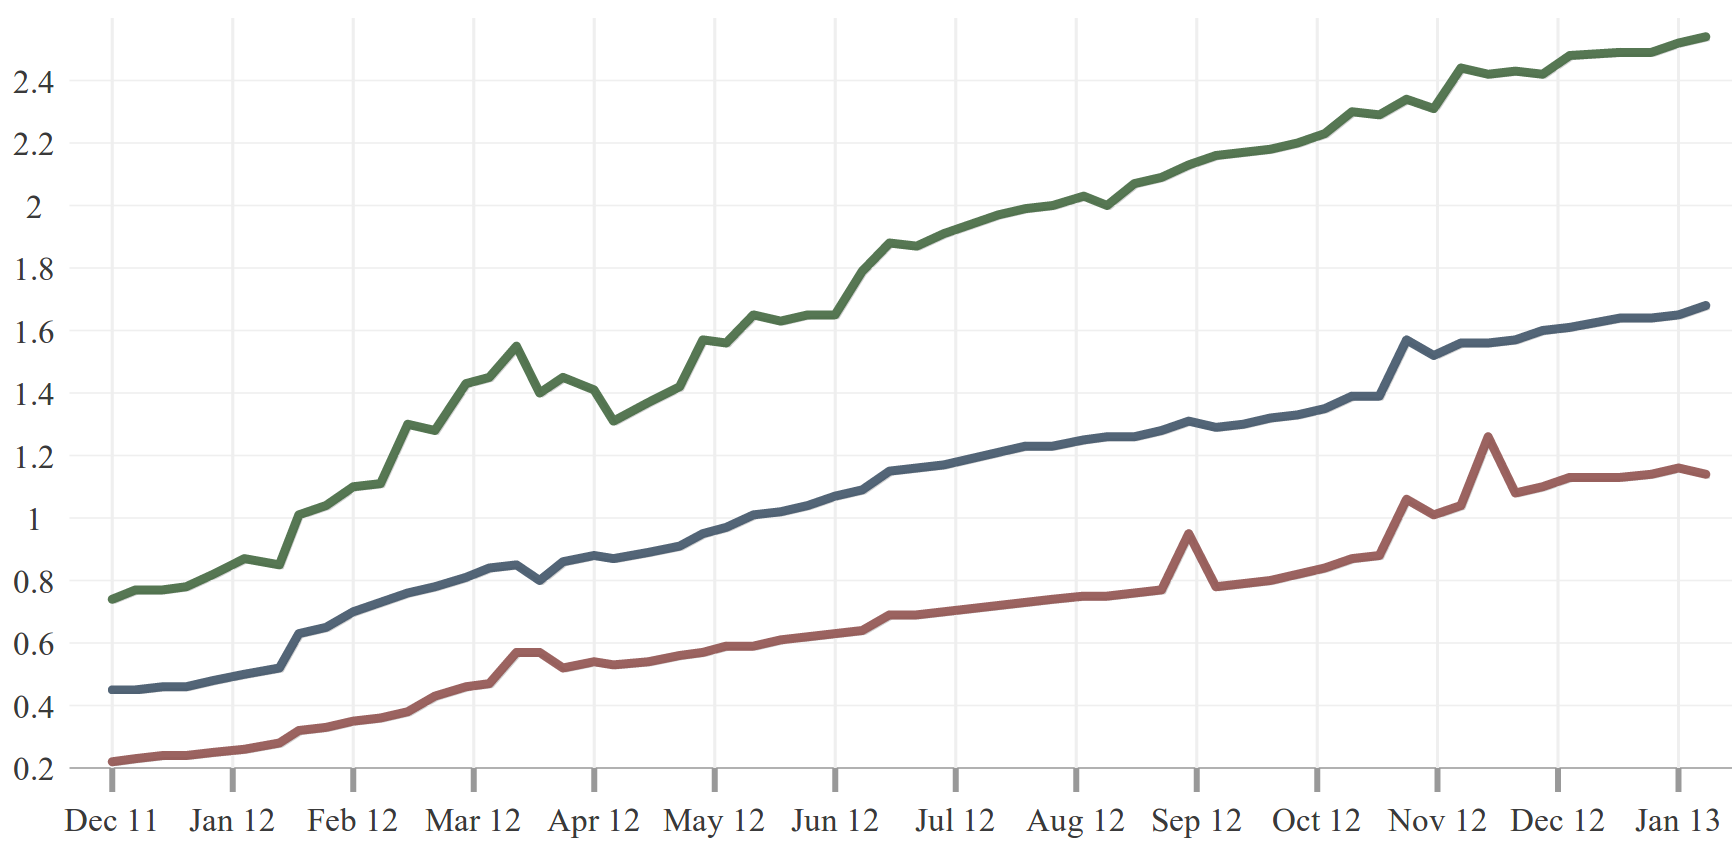
\includegraphics[width=13cm]{md-chart}
    \caption{Usage statistics for Microdata.\cite{mdStat} The values represend
    procentages of usage for the top 10,000 websites (green), top 100,000 (blue)
    and top million (red).}
    \label{mdChart}
\end{figure}


\begin{description}
    \item[Green Turtle] is a library and a Chrome extension which provides the
    RDFa API on every page and a triples viewer;\cite{greenTurtle}
    \item[RDF Detective] is a extension for Chrome which detects RDF annotations
    embedded in HTML pages and can open them in an external
    viewer.\cite{rdfDetective}
\end{description}

\subsection{Microdata}

Microdata is a WHATWG HTML specification which adds new attributes to HTML5 for
embedding sematics into web pages.\cite{mdWiki}

Microdata provides a simpler way for annotating HTML elements than RDFa, but it
is also less powerful.

One of its advantages is that it primarily uses the \co{schema.org} vocabulary
which is comprehensive and consistent and supported by the three largest search
engines. Acording to a statistic\cite{mdStat}, which is graphed in
Figure~\ref{mdChart}, it is more used than RDFa and it is adopted at a faster
rate.

\begin{figure}[t!]
    \centering
    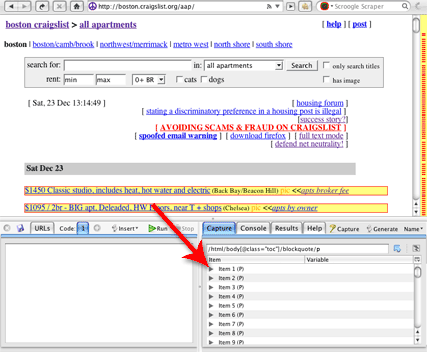
\includegraphics[width=8cm]{piggy}
    \caption{Example solvent in Piggy Bank from its website.}
    \label{pbSolvent}
\end{figure}

Extensions:

\begin{description}
    \item[SchemaDump] is an extension for Chrome which parses microdata on a
    page and shows is in a tabular form\cite{schemaDump}.
\end{description}

\subsection{Other sematic web extensions}

\textbf{Piggy Bank} is a Firefox extension which harvests data as a user
browses. It allows the browser to become a mashup platform by mixing extracted
data. Collected data can be saved locally and interacted with
afterwards.\cite{piggyBank}

It can be used to write smarter scrapers with a few lines of JavaScript. Since
data is marked up sematically the quality of extracted information is higher and
extraction ca be automated easier for example by using solvent as shown in
Figure~\ref{pbSolvent}.

\section{Implementation}

\subsection{Libraries used}

\begin{figure}[b!]
    \centering
    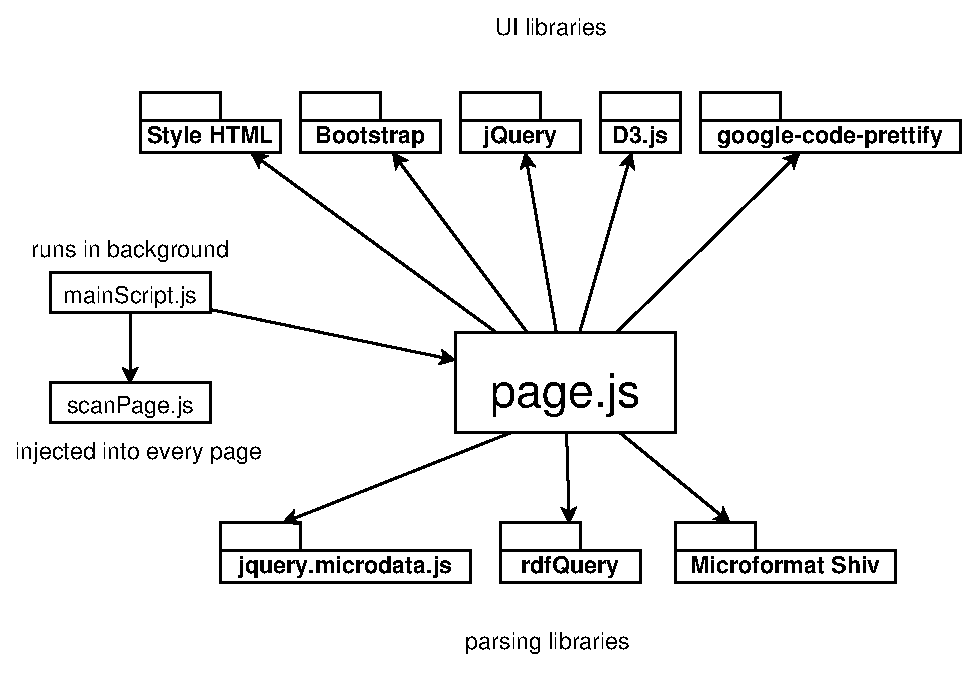
\includegraphics[width=13cm]{diagram}
    \caption{The architecture of the extension.}
    \label{sysArch}
\end{figure}

Figure~\ref{sysArch} shows architecture of the extension. The following
libraries are used:

\begin{description}
    \item[rdfQuery] for extracting RDFa;
    \item[Microformat Shiv] for extracting microformats;
    \item[jquery.microdata.js] for extracting Microdata (this jQuery plugin
    mimics the Microdata DOM API that Chrome doesn't have so far);
    \item[jQuery] for controlling the UI easier;
    \item[Bootstrap] (CSS and JavaScript) for good looking and adaptable UI;
    \item[D3.js] for displaying the interactive graph;
    \item[google-code-prettify] for colorizing the source HTML;
    \item[Style HTML] for autoformatting the source HTML and RDF/XML.
\end{description}

\subsection{Background page}

When the browser is started, a background page is opened and \co{mainScript.js}
is loaded in it. This small script listens for tabs openning, reloding and
closing. When a new tab has finished loading, \co{scanPage.js} is injected into
it. This script scans the DOM for the presence of the three formats and returns
that to the background script.

If any formats are found a page actions icon is opened (an icon at the right of
the address bar) which also shows what was found.

The purpose of this design is so that the extension won't be obtrusive or too
resource demanding.

\subsection{Content page}

If the user clicks on the icon, a new tab is opened which will contain all the
content.

Depending on the detected formats, the necessary scripts will be inserted into
the original tab in order to extract the needed data.

Most of the operations are split with timeouts so that the browser can show the
intermediary steps before all the operations are finished.

The first item on the page is the autoformatted and syntax highlighted source
HTML page. In it, attributes specific to RDFa and Microdata ar highlighted in
yellow.

\begin{figure}[t!]
    \centering
    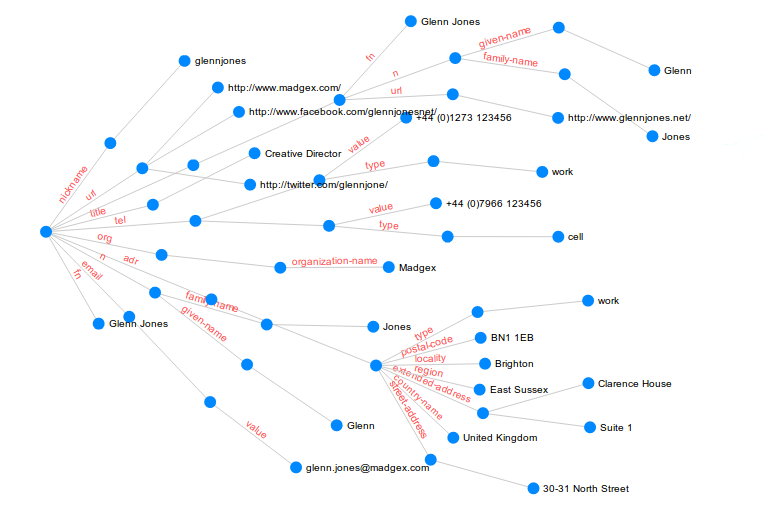
\includegraphics[width=13cm]{tree}
    \caption{Example tree generated from an hCard.}
    \label{treeEx}
\end{figure}

If Microdata is detected \co{jquery.microdata.js} is used to extract it all in a
way specific to what \co{document.getItems()} should return.

That is processed by in order to obtain the RDF/XML and Turtle. These are
written by me.

If RDFa is detected \co{rdfQuery} is used to obtain the RDF/XML and the JSON
triples (not JSON-LD). The RDF/XML file returned isn't completly correct so I
process it again. I wrote the conversion to Turtle and CSV triples.

If Microformats are detected I use Microformat Shiv to extract the data and
convert it to RDF/XML. I also make a tree structure out of the data and display
it with D3.js which allows for interaction. Figure~\ref{treeEx} shows an
example.

\section{Use cases}

This extension is intended to be used for developers who want to visualize and
test the metadata on their pages or to learn/see how others are using
microformats, Microdata and RDFa.

For example one could use the extension to view Microdata automatically entered
into a page by various libraries and it can be saved locally as an RDF file to
be used by other tools.

Figure~\ref{sourceView} is showing the highlighted usage of Microdata attributes
in the autoformatted source code of a page. Pages created by web application
frameworks are harder to inspect by just looking at the normal output.

Figure~\ref{rdfView} is showing the RDF extracted from such a page and how it
can be saved.

\begin{figure}[t!]
    \centering
    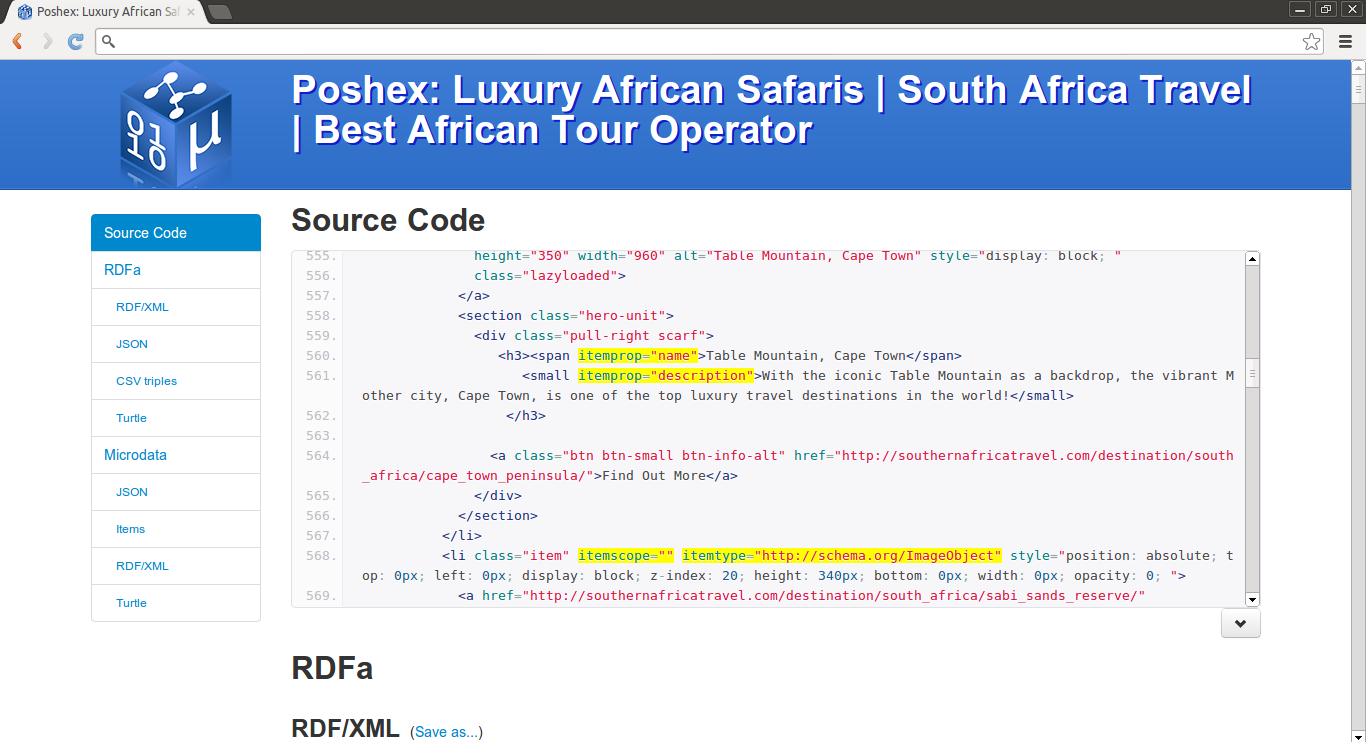
\includegraphics[width=13cm]{source-view}
    \caption{How the newly opened tab looks.}
    \label{sourceView}
\end{figure}

\begin{figure}[t!]
    \centering
    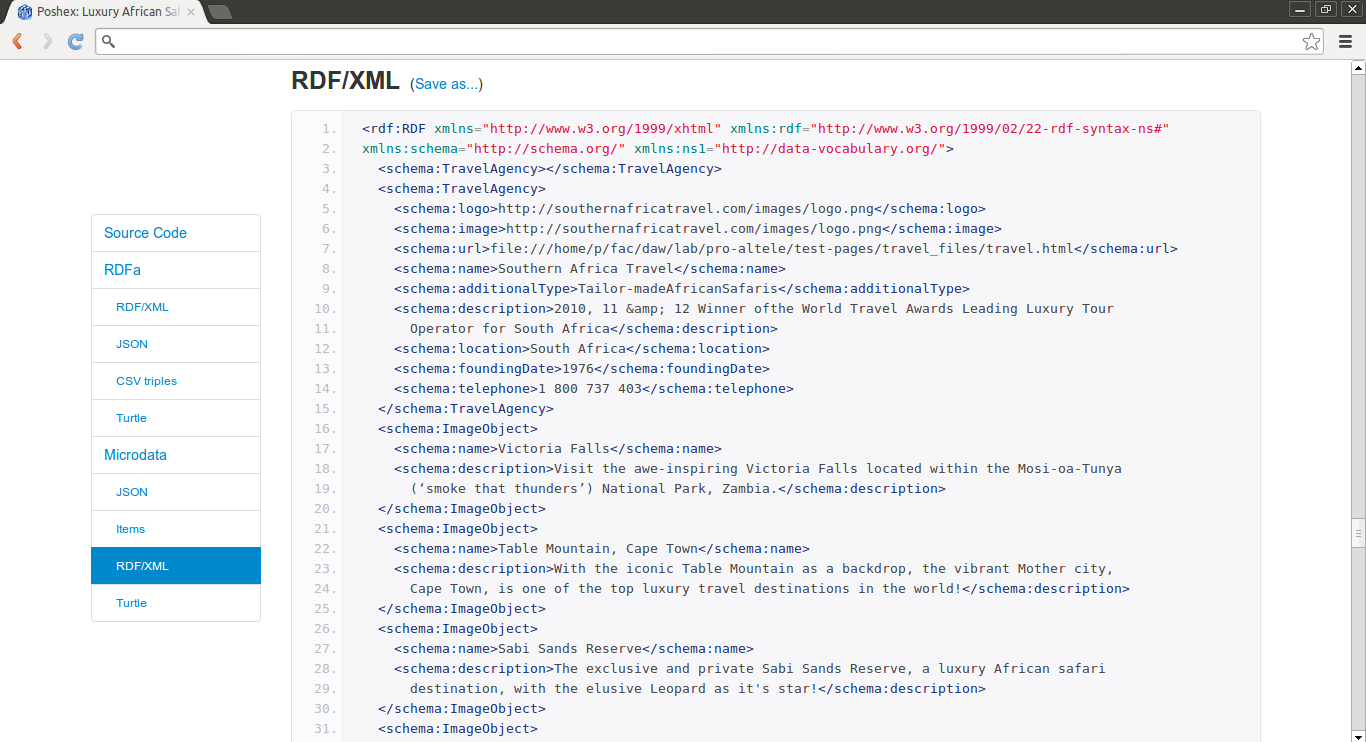
\includegraphics[width=13cm]{rdf-view}
    \caption{How RDF/XML is displayed.}
    \label{rdfView}
\end{figure}

\section{Conclusions and future work}

Given that Microdata and RDFa are better formats for structured data on the web
a tool such as this can help convert data from pages with microformats. But it
can also be used to inspect such data.

This extension can be improved by writing more convertors and using D3.js for
other visualizations.

Microformats to RDF (XML/Turtle) can be improved by adding more mappings to RDF
classes and properties. I only implemented hCard conversion extensively by
mapping it to three ontologies: FOAF, VCard and W3C PIM as show in a
recomandation\cite{mappings}.

\addcontentsline{toc}{section}{References}
\begin{thebibliography}{9}
    \bibitem{ufHist} \texttt{http://microformats.org/wiki/history-of-microformats}
    \bibitem{ufWiki} \texttt{http://en.wikipedia.org/wiki/Microformat}
    \bibitem{ufStat} \texttt{http://webdatacommons.org/}
    \bibitem{ufExt} \texttt{http://microformats.org/wiki/firefox-extensions}
    \bibitem{rdfaWiki} \texttt{http://en.wikipedia.org/wiki/RDFa}
    \bibitem{rdfaStat} \texttt{http://trends.builtwith.com/docinfo/XHTML-RDFa-1.0}
    \bibitem{greenTurtle} \texttt{http://code.google.com/p/green-turtle/}
    \bibitem{rdfDetective} \texttt{https://chrome.google.com/webstore/detail/}
        \texttt{rdf-detective/ghenajlebmgkoohljekdpahbnejiijfm}
    \bibitem{mdWiki} \texttt{http://en.wikipedia.org/wiki/Microdata\_(HTML)}
    \bibitem{mdStat} \texttt{http://trends.builtwith.com/docinfo/Microdata}
    \bibitem{schemaDump} \texttt{https://chrome.google.com/webstore/detail/}
        \texttt{schemadump/melmflpcmnoddilkindbepcbcjbjbdin}
    \bibitem{piggyBank} \texttt{http://simile.mit.edu/wiki/Piggy\_Bank}
    \bibitem{mappings} \texttt{http://www.ibiblio.org/hhalpin/homepage/notes/vcardtable.html}
\end{thebibliography}

\end{document}
